\clearpage
\section{Osnovni pojmovi i sistemi u igrama}
\label{sec:Section_Name}

\subsection{Game Loop}
Klju\v{c}na ta\v{c}ka izvr\v{s}avanja igre jeste glavna petlja igre (eng. game loop).
Jednom kada je igra pokrenuta sve ono \v{s}to je vidljivo korisniku, grafika, 
zvuk, interakcija procesira se kroz glavnu petlju. U tom jednom prolazu petlje koji
nazivamo \emph{tick} ili \emph{frame} de\v{s}ava se iscrtavanje grafike, reagovanje na 
korisni\v{c}ki unos (unos sa tastature ili putem mi\v{s}a ili nekih drugih perifernih ure\dj aja) 
te reakcija sveta na zadate promene... odnosno, ovde se de\v{s}ava sve, zato je glavna 
petlja srce same igre. Modernije arhitekture dozvoljavaju odre\dj eni stepen paralelizacije
nekih procesa, pa bi na primer iscrtavanje grafike moglo da se izdvoji u paralelan proces i sli\v{c}no.

\subsubsection{FPS}
FPS skra\'ceno od \emph{frames per second} je osnovna mera performansi igre. Ova mera kazuje nam
koliko je puta po sekundi mogu\'ce izvr\v{s}iti glavnu petlju. Ve\'ci broj je i bolji, pa tako igra
koja se izvr\v{s}ava na manje od 30 frejmova po sekundi nije prijatna za igranje
i doga\dj a se takozvano \emph{seckanje}, odnosno objekti se ne pomeraju glatko kako bi trebalo
ve\'c iscepkano \v{s}to naru\v{s}ava celokupan do\v{z}ivljaj igranja. Nizak FPS mo\v{z}e
da bude rezultat lo\v{s}e napisanog koda ili prosto zastarelog hardvera. Moderne igre se trude da 
se odr\v{z}e na 60 FPS.

\subsubsection{Update}
Update je funkcija koja se poziva upravo iz glavne petlje igre. To je funkcija koja je mo\v{z}e biti
definsana u MonoBehavior klasi. Update funkcija se poziva nad svakim objektom tipa MonoBehavior (ukoliko
je defini\v{s}e) ta\v{c}no jednom svakog frejma \cite{unitydocs}. Sva promenljiva pona\v{s}anja objekta
mogu se definisati ovde.

\subsubsection{FixedUpdate}
Sli\v{c}no funkciji Update, i ova funkcija se poziva periodi\v{c}no ali ne svakog frejma, ve\'c 
na fiksno vreme svake 0.02 sekunde \cite{unitydocs}. Prema uputstvima iz dokumentaicje,
u ovoj funkciji se mora raditi sve \v{s}to ima veze sa bilo kakvim izra\v{c}unavanjem fizike. U igri
se oslanjamo na Unity-jev sistem za fiziku za kretanje, pa \'cemo se dalje u tekstu detaljnije
baviti time.

\subsubsection{Vremena, klasa Time}
Jedna od bitnijih stavki u igrama jeste vreme. Merimo dve vrste vremena, koja o\v{c}itavamo iz klase \emph{Time}.

\emph{Time.time} je vreme koje je proteklo od pokretanja igre i ono je korisno
obi\v{c}no kada \v{z}elimo da ograni\v{c}imo izvr\v{s}avanje nekog dela koda vremenski.
Na primer, ne \v{z}elimo da neprijatelji prebrzo ispaljuju metke na igra\v{c}a, te mo\v{z}emo meriti
vreme proteklo od prethodnog pucanja i proveriti da li je to vreme ve\'ce od neke konstante
koja nam predstavlja minimalan vremenski interval izme\dj u dva pucnja.

\emph{Time.deltaTime} je vreme za koje se izvr\v{s}io prethodni frejm. Ovo je jako bitna stavka,
i potrebno nam je kada imamo bilo kakvu promenu stanja u igri koja je vidljiva (na primer, kretanje). Kako se u glavnoj petlji
izvr\v{s}ava svaka takva promena, to znav\v{c}i da se promena de\v{s}ava jednom po frejmu. Ve\'c je pomenuto
da moderne igre te\v{z}e ka konstantnom izvr\v{s}avanju na 60 FPS ali to nije uvek mogu\'ce, odnosno de\v{s}ava
se da zbog lo\v{s}ijeg hardvera ili lo\v{s}eg koda FPS opada.

Uzmimo kao primer kretanje nekog objekta. Tada imam vektor $v$ koji je vektor pomeraja u svakom
frejmu. Zbog nekonzistentnosti FPSa na razli\v{c}itim ra\v{c}unarima postoji opasnost da dobijemo razli\v{c}ite 
brzine kretanja, ovo je problem koji direktno naru\v{s}ava mogu\'cnost igranja na zami\v{s}ljen na\v{c}in,
posebno u multiplayer igrama. Pogledati ~\ref{fig:deltatime} za ilustraciju. 

\begin{center}
    \begin{figure}
        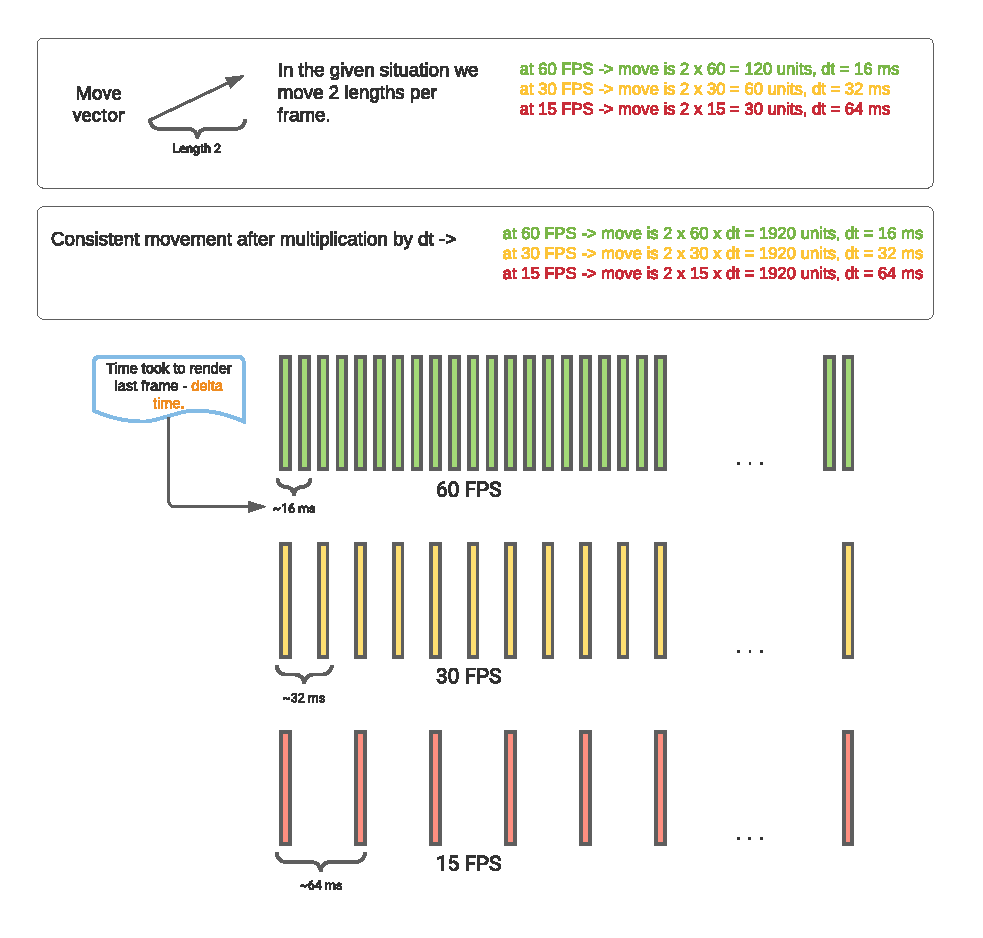
\includegraphics[width=1\textwidth]{Figures/DeltaTime.pdf}
        \caption{DeltaTime obja\v{s}njenje}
        \label{fig:deltatime}
    \end{figure}
\end{center}

\subsection{Obrasci (eng. design patterns)}
U razvoju softvera a posebno kompleksnijih sistema i ve\'cih projekata \v{c}esto se sre\'ce upotreba raznih
obrazaca koji olak\v{s}avaju organizaciju koda i poma\v{z}u da se razre\v{s}e nepotrebna uplitanja (eng. coupling)
izme\dj u klasa. Obrasci su tu da nadomeste nedostatke nekih programskih jezika.

\subsubsection{"Singleton" obrazac}
Ovaj obrazac osigurava da postoji ta\v{c}no jedna instanca singleton klase, kao i mogu\'cnost globalnog pristupa toj instanci \cite{gameprog}.
Ostale prednosti kori\v{s}\'cenja ovog obrasca su:

\begin{itemize}
    \item Instanca klase se ne pravi ukoliko se ne koristi.
    \item Inicijalizacija se de\v{s}ava tokom izv\v{s}avanja programa (izbegavamo kori\v{s}\'cenje \v{c}isto stati\v{c}kih klasa).
    \item Klasa mo\v{z}e biti nasle\dj ena. 
\end{itemize}

Primer implementacije Singleton obrasca koji nije thread-safe (lo\v{s}e)!
\begin{verbatim}
    public class Singleton
    {
        private static Singleton _instance = null;

        private Singleton() { }

        public static Singleton Instance
        {
            get
            {
                if (_instance == null)
                {
                    _instance = new Singleton();
                }
                
                return _instance;
            }
        }
    }
\end{verbatim}

Jednostavna thread-safe implementacija:
\begin{verbatim}
    public class Singleton
    {
        private static Singleton _instance = null;
        private static readonly object _root = new object();

        Singleton() { }

        public static Singleton Instance
        {
            get
            {
                lock (_root)
                {
                    if (_instance == null)
                    {
                        _instance = new Singleton();
                    }

                    return instance;
                }
            }
        }
    }
\end{verbatim}

U Unity platformi postoje situacije kada se neki problemi ne mogu re\v{s}iti pomo\'csu stati\v{c}kih klasa, 
stoga moramo koristiti Singleton kako bi smo osigurali globalni pristup ali pri tome sa\v{c}uvati osobine MonoBehavior-a. 
Primer takve klase je klasa \emph{GameManager} o kojoj \'ce biti vi\v{s}re re\v{c}i dalje u tekstu. Implementacija Singleton obrasca se 
u Unity platformi dodatno razlikuje, jer komponente koje su izvu\v{c}ene na scenu vizuelno, ve\'c jesu instance tih klase, ali to se lako re\v{s}ava,
\v{s}to \'cemo videti na prilo\v{z}enom kodu (izvor github.com):

\begin{verbatim}
/// <summary>
/// Mono singleton Class. Extend this class to make singleton component.
/// Example: 
/// <code>
/// public class Foo : MonoSingleton<Foo>
/// </code>. To get the instance of Foo class, use <code>Foo.instance</code>
/// Override <code>Init()</code> method instead of using <code>Awake()</code>
/// from this class.
/// </summary>
public abstract class MonoSingleton<T> : MonoBehaviour where T : MonoSingleton<T>
{
    private static T m_Instance = null;
    public static T Instance
    {
        get
        {
            // Instance requiered for the first time, we look for it
            if (m_Instance == null)
            {
                m_Instance = GameObject.FindObjectOfType(typeof(T)) as T;

                // Object not found, we create a temporary one
                if (m_Instance == null)
                {
                    Debug.LogWarning("No instance of " + typeof(T).ToString() + ", a temporary one is created.");

                    isTemporaryInstance = true;
                    m_Instance = new GameObject("Temp Instance of " + typeof(T).ToString(), typeof(T)).GetComponent<T>();

                    // Problem during the creation, this should not happen
                    if (m_Instance == null)
                    {
                        Debug.LogError("Problem during the creation of " + typeof(T).ToString());
                    }
                }
                if (!_isInitialized)
                {
                    _isInitialized = true;
                    m_Instance.Init();
                }
            }
            return m_Instance;
        }
    }

    public static bool isTemporaryInstance { private set; get; }

    private static bool _isInitialized;

    // If no other monobehaviour request the instance in an awake function
    // executing before this one, no need to search the object.
    private void Awake()
    {
        if (m_Instance == null)
        {
            m_Instance = this as T;
        }
        else if (m_Instance != this)
        {
            Debug.LogError("Another instance of " + GetType() + " is already exist! Destroying self...");
            DestroyImmediate(this);
            return;
        }
        if (!_isInitialized)
        {
            DontDestroyOnLoad(gameObject);
            _isInitialized = true;
            m_Instance.Init();
        }
    }


    /// <summary>
    /// This function is called when the instance is used the first time
    /// Put all the initializations you need here, as you would do in Awake
    /// </summary>
    public virtual void Init() { }

    /// Make sure the instance isn't referenced anymore when the user quit, just in case.
    private void OnApplicationQuit()
    {
        m_Instance = null;
    }
}
\end{verbatim}

\subsubsection{"Command" obrazac}
Ovaj obrazac slu\v{z}i da delegira izvr\v{s}avanje neke funkcije te tako omogu\'ci da se izbegne 
pojam \emph{hardwire} odnosno \v{c}vrsto vezivanje izme\dj u nekih entiteta, na primer, \v{c}itanja 
korisnikovog unosa sa tastature te reagovanje na isti. Uzmimo ba\v{s} taj primer:

\begin{verbatim}
    void HandleInput()
    {
        if (isPressed(BUTTON_X)) Jump();
        else if (isPressed(BUTTON_Y)) FireGun();
        else if (isPressed(BUTTON_A)) SwapWeapon();
        // ...
    }
\end{verbatim}

Ukoliko \v{z}elimo da druga\v{c}ije mapiramo komande, \v{s}to je vrlo \v{c}est slu\v{c}aj u igrama, 
kroz konfiguracioni meni. Za na\v{s}e potrebe napravi\'cemo apstraktnu klasu \emph{ACommand}.

\begin{verbatim}
    
    public abstract class ACommand
    {
        public KeyState State { get; set; }
        public bool IsPhysics { get; private set; }

        public ACommand(bool isPhysics)
        {
            IsPhysics = IsPhysics;
        }

        public abstract void Execute(ShipController ship, Actor actor);
    }
\end{verbatim}

Dalje prema potebama nasle\dj ujemo ovu klasu i defini\v{s}emo konkretna pona\v{s}anja. Na primer,
dodavanje potiska:

\begin{verbatim}
    public sealed class Thrust : ACommand
    {
        public Thrust() : base(true) { }

        public override void Execute(ShipController ship, Actor actor)
        {
            ship.AddThrust(ship.transform.up, actor.ThrustPower);
        }
    }
\end{verbatim}

Ove komande se onda pakuju u neku strukturu, u na\v{s}em slu\v{c}aju koristimo \emph{Queue}, 
i procesiramo ih u glavnoj petlji. Ovo radimo ovako, jer ho\'cemo da registrujemo i po nekoliko
unosa istovremeno, odnosno, na primer, brod mo\v{z}e da se kre\'ce napred i da puca istovremeno.

\begin{verbatim}
    while (actions.Count > 0)
    {
        var action = actions.Dequeue();
        action.Execute(this, _actor);
    }
\end{verbatim}

Po\v{s}to smo napravili ovakvu apstrakciju, sada je mogu\'ce da i pona\v{s}anje neprijatelja
zadajemo preko komandi, odnosno skripta koja kontrli\v{s}e neprijatelja \'ce samo dodavati potrebne
akcije u niz akcija. Na primer, kretanje prema igra\v{c}u:

\begin{verbatim}
    // Move towards player target
    Vector2 targetDir = _target.position - transform.position;
    if (targetDir.magnitude >= 5f)
    {
        actions.Enqueue(new Thrust());
    }
\end{verbatim}

Na drugoj strani, kod igra\v{c}a, defini\v{s}emo akcije kao mapu:

\begin{verbatim}
    InputManager.Instance.InputMap[KeyCode.UpArrow] = new Thrust();
    InputManager.Instance.InputMap[KeyCode.LeftArrow] = new Rotate(1);
    InputManager.Instance.InputMap[KeyCode.RightArrow] = new Rotate(-1);
    InputManager.Instance.InputMap[KeyCode.LeftControl] = new Shoot(AmmoType.DEFAULT,
        new Vector2[]
        {
            Vector3.up * 1.5f
        });
\end{verbatim}

a onda u klasi koja se bavi u\v{c}itavanjem unosa sa tastature imamo slede\'ce:

\begin{verbatim}
    foreach (var input in InputMap)
    {
        if (Input.GetKeyDown(input.Key))
        {
            input.Value.State = KeyState.PRESSED;
            inputQueue.Enqueue(input.Value);
        }

        else if (Input.GetKey(input.Key))
        {
            input.Value.State = KeyState.HELD;
            inputQueue.Enqueue(input.Value);
        }
    }
\end{verbatim}

Postavlja se pitanje da li bi onda i akcije Thrust, Rotate (mo\v{z}a dodatno RotateLeft i RotateRight) mogle da budu
Singleton objekti, i odgovor je pozitivan ali sa nekim odre\dj enim izmenama, ali time se ne\'cemo baviti dublje.
